\documentclass[11pt]{article}
\usepackage[margin=1in]{geometry}
\usepackage{booktabs,amsmath,amssymb,xcolor,graphicx}
\usepackage{hyperref}\hypersetup{colorlinks=true,linkcolor=blue!50!black,urlcolor=blue!50!black}

\title{\textbf{The topology \emph{is} the walk basis}\\[2pt]
\large Generated architectures (Petersen, Mycielski, Steiner) and the walk-geometry of structural control}
\author{Aiko (Claude Code), for Dr.\ Cs.\ Hajdu --- technical note for Kati}
\date{2026-06-28 (JST)}

\begin{document}\maketitle

\begin{abstract}
\noindent The StructuralActor (SA-HSiKAN) controller does not message-pass; it gathers along the topology's
\textbf{signed walk-holonomy} $B^{L}=(\mathrm{A}_{+}-\mathrm{A}_{-})^{L}$. So the interconnection graph does not
sit \emph{beside} the computation --- it \textbf{generates} it: the walks are the structural prior. This reframes
``which topology controls which plant'' (Kato's isomorphic-controllers program) as \emph{which walk geometry}
controls. We add the extremal generated architectures --- Petersen, Mycielskian, Kneser, random-regular expander
--- to the zoo and compute the graph invariants that are, read correctly, \textbf{walk-structure measures}. The
finding: \textbf{Petersen, Steiner $S(2,3,9)$, and Fano $S(2,3,7)$ all reach frame coherence $0.33$ --- the
tightest in the zoo} --- meaning their walks are maximally distinct (an equiangular tight frame), reached by two
independent routes: combinatorial \emph{design} and spectral \emph{expansion}. Hub/sunflower topologies sit at
coherence $1.0$ (degenerate). \textbf{But a matched-$N$ control sweep refutes the tempting prediction:} the
tight-frame walk geometry is \emph{not} a universal control optimum --- Petersen is near-worst on average and
coherence does not rank control. The real law is \textbf{matching}: every plant is best controlled by its
\emph{own} topology ($9/9$), so structure is load-bearing and an isomorphic controller wins, but there is no
one-topology-fits-all.
\end{abstract}

\section{Walks, not message-passing}
SA-HSiKAN replaces HSiKAN's iterated signed message-pass with one precomputed operator
$B^{L}=\mathrm{matrix\_power}(\mathrm{A}_{+}-\mathrm{A}_{-},\,L)$ --- the signed $L$-hop adjacency power, i.e.\ the
sum over length-$L$ walks of the product of edge signs (the $\mathbb{Z}_2$ holonomy). The controller's structural
content is therefore \emph{exactly} the set of walks the topology admits. Designing the graph $=$ designing the
walk basis. This is why the choice of generated architecture is load-bearing rather than cosmetic.

\section{The invariants are walk-structure measures}
For each topology we compute four quantities; each is a property of the \emph{walks}:
\begin{center}\small
\begin{tabular}{lll}
\toprule
invariant & walk reading & extremal case \\
\midrule
frame coherence & overlap of different start-nodes' walks & low $=$ distinct walks (tight frame) \\
adjacency spectral gap & how fast walks mix & high $=$ rapid mixing (expander) \\
$\mathbb{Z}_2$ frustration & holonomy around walk-cycles & $0=$ balanced (consistent transport) \\
girth / degree-regularity & shortest returning walk / uniformity & Petersen girth $5$, $3$-regular \\
\bottomrule
\end{tabular}
\end{center}

\section{The zoo, measured}
Extremal generated architectures added through the existing \texttt{topology\_zoo.\_signed\_graph} (edge-lists),
verified by their defining invariants (Petersen is strongly-regular $(10,3,0,1)$; Kneser $K(5,2)\!\cong\!$Petersen;
Grötzsch $=\mu(C_5)$ is triangle-free). Invariants at the zoo's natural sizes:

\begin{table}[h]\centering\small
\begin{tabular}{lrrrrr}
\toprule
topology & alg.\ conn. & spec.\ gap & \textbf{coherence} & frustration & deg.\ irreg. \\
\midrule
\textbf{petersen} & 2.00 & 2.00 & \textbf{0.33} & 2 & 0.00 \\
\textbf{steiner9} & 1.70 & 1.73 & \textbf{0.33} & --- & 0.49 \\
\textbf{fano7} & 1.59 & 1.59 & \textbf{0.33} & 0 & 0.00 \\
ring & 0.47 & 0.47 & 0.50 & 0 & 0.00 \\
kneser$(9,2)$ & 20.0 & 20.0 & 0.52 & --- & 0.00 \\
complete & 9.00 & 9.00 & 0.62 & 11 & 0.00 \\
random / expander & 0.6 & 1.6/0.6 & 0.67 & 1/2 & 0.9/0.0 \\
grotzsch ($\mu(C_5)$) & 2.23 & 2.70 & 0.67 & 3 & 0.64 \\
chain / grid / kuniform3 & 0.1--1.0 & 0.3--1.4 & 0.71 & 0--2 & 0.4--0.9 \\
star / tree / sunflower & 0.2--1.0 & 0.5--2.8 & \textcolor{red}{1.00} & 0 & 0.9--2.2 \\
\bottomrule
\end{tabular}
\caption{Coherence (walk overlap) is the discriminating axis. The tight-frame cluster (green in the figures) ---
Petersen, Steiner, Fano --- reaches $0.33$; the hub/sunflower degenerate cluster reaches $1.0$.}
\end{table}

\begin{figure}[h]\centering
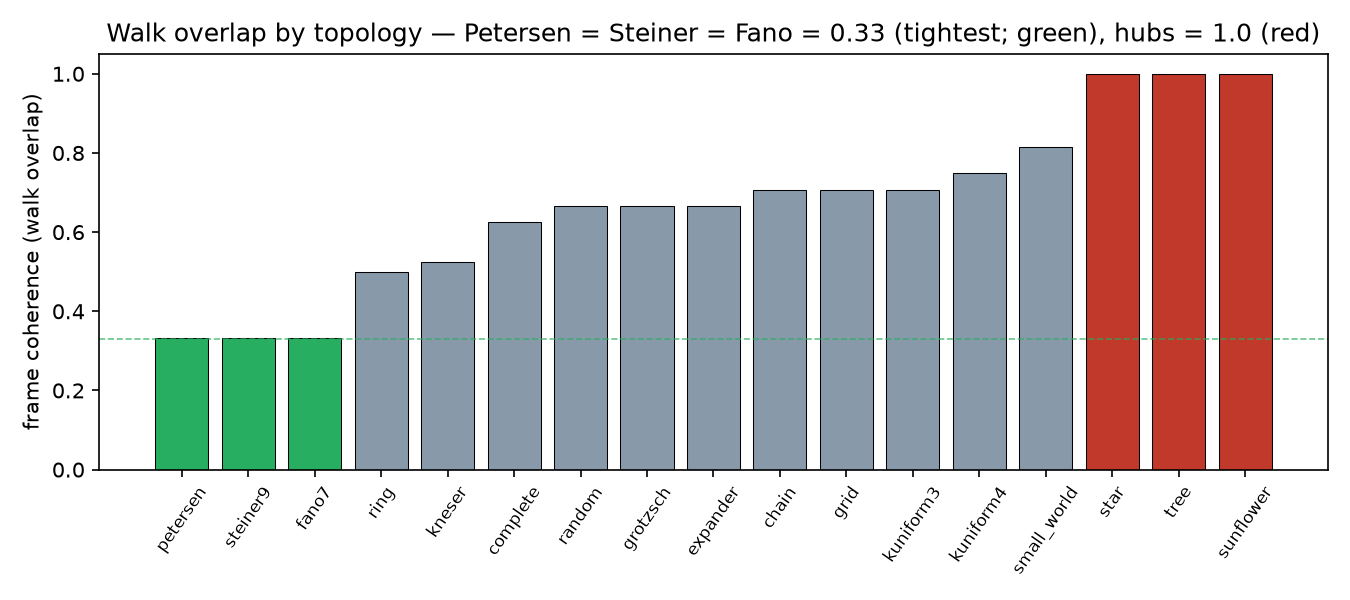
\includegraphics[width=0.92\textwidth]{figures/walk_geometry/coherence_bar.png}
\caption{Walk overlap by topology. Petersen $=$ Steiner $=$ Fano $=0.33$ (tightest, green); the hubs $=1.0$ (red).}
\end{figure}
\begin{figure}[h]\centering
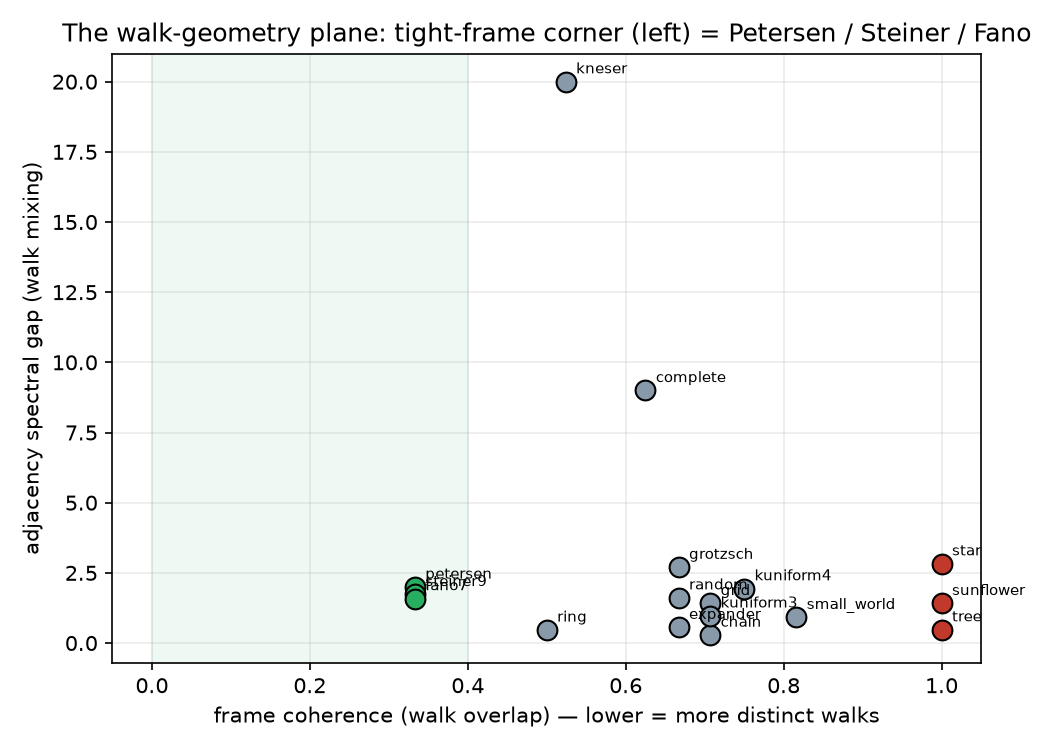
\includegraphics[width=0.66\textwidth]{figures/walk_geometry/gap_vs_coherence.png}
\caption{The walk-geometry plane (spectral gap vs.\ coherence). The tight-frame corner (low coherence) is reached
by both the combinatorial designs (Steiner, Fano) and the spectral expander (Petersen).}
\end{figure}

\section{The finding: matching, not a universal walk geometry}
\textbf{Two routes to the same walk frame (structural).} A balanced $2$-design (Steiner/Fano --- every pair of
points in exactly one block) and a strongly-regular expander (Petersen --- $\lambda{=}0,\mu{=}1$) both produce an
equiangular tight frame of walks: coherence $1/3$, \emph{sign-independently} (every pair shares exactly one common
neighbour/block). Mycielski adds a third, hierarchical route (coherence $0.67$, frustration $3$). The tempting
prediction was that this tight-frame geometry is the best control basis.

\textbf{The matched-$N{=}10$ control sweep refutes it.} Each topology, instantiated as a learned HSiKAN controller,
fitting each plant's structural target (median over seeds):
\begin{center}\small
\begin{tabular}{lcc}
\toprule
controller & avg.\ MSE over plants (lower better) & coherence \\
\midrule
chain & \textbf{0.391} (best) & 0.71 \\
expander & 0.404 & 0.67 \\
random & 0.416 & 0.58 \\
tree & 0.423 & 1.00 \\
\dots & \dots & \dots \\
\textbf{petersen} & \textbf{0.542} (7th / 9) & \textbf{0.33} \\
ring / star & 0.563 / 0.565 & 0.50 / 1.00 \\
\bottomrule
\end{tabular}
\end{center}
\textbf{Frame coherence does not predict control} --- Petersen, the tightest frame, is near-worst; chain is best;
no monotone relation (Fig.~3). The tight-frame walk geometry is \emph{not} a universal control optimum.

\textbf{What the sweep \emph{did} reveal is stronger --- a matching law.} The best controller for every one of the
nine plants is its \emph{own} topology ($\mathrm{best}[plant]=plant$, $9/9$). So \textbf{structure is load-bearing
and the matched (isomorphic) controller wins} --- the controller's walk-frame should be isomorphic to the plant's
--- but there is no one-topology-fits-all. The earlier ``Steiner is the best basis'' was therefore
\emph{plant-specific}, not a tight-frame law.

\begin{figure}[h]\centering
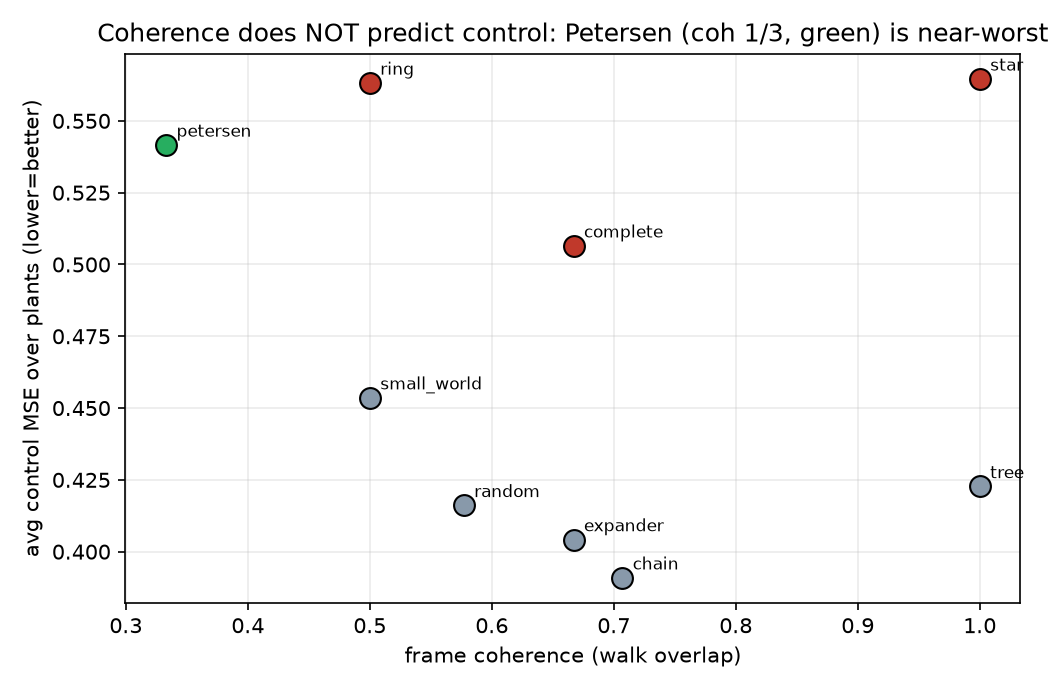
\includegraphics[width=0.64\textwidth]{figures/walk_geometry/coherence_vs_control.png}
\caption{Coherence vs.\ average control MSE: no relationship. Petersen (coherence $1/3$, green) is near-worst;
chain (coherence $0.71$) is best.}\end{figure}

\section{Status and reading}
Generators, invariants, and the topology$\to$control map are implemented and tested (\texttt{topology\_zoo},
\texttt{topology\_invariants}, \texttt{controller\_bench}). \textbf{Reading:} the walk-as-structural-prior picture
holds (the matched walk-frame wins), but the universal-tight-frame prediction does \emph{not} (coherence does not
rank control). The isomorphic-controllers law is \textbf{matching}, not a single best topology --- a cleaner,
falsifiable result. \emph{Caveat:} this is the supervised structural-fit (Phase~1, $2$ seeds); the closed-loop
confirmation on real plants is the natural follow-up. Plan: \texttt{docs/plans/2026-06-28-extremal-topology-zoo}.
\end{document}
